\begin{surferPage}[A3+- Singularität]{Eine $A_3^{+-}$ Singularität}
Eine $A_3^{+-}$ Singularität sieht einer Cuspe der Form $A_2^{+-}$ mit
    Gleichung $x^3+y^2-z^2$ sehr ähnlich; nur ist sie zusätzlich symmetrisch
    zur $yz$- Ebene: 
    \[x^4+y^2-z^2=0.\]
    Die damit insgesamt drei Spiegel - Symmetrien zu den drei Koordinaten - Ebenen
    kann man an der Gleichung 
    recht einfach erkennen; 
    es gilt nämlich:
    \[(-x)^4+y^2-z^2=x^4+y^2-z^2\] 
    und analog für die anderen Variablen: $y\mapsto -y$ und $z\mapsto -z$. 

    Eine ebene $A_3^{+-}$ Singularität kann man, ähnlich wie die Cuspe in der
    Kaffee - Tasse, sehen, wenn Sonnenlicht durch ein Teeglas fällt:
    \vspace*{-0.5em}
    \begin{center}
      \begin{tabular}{c@{\qquad}c}
        \begin{tabular}{@{}c@{}}
          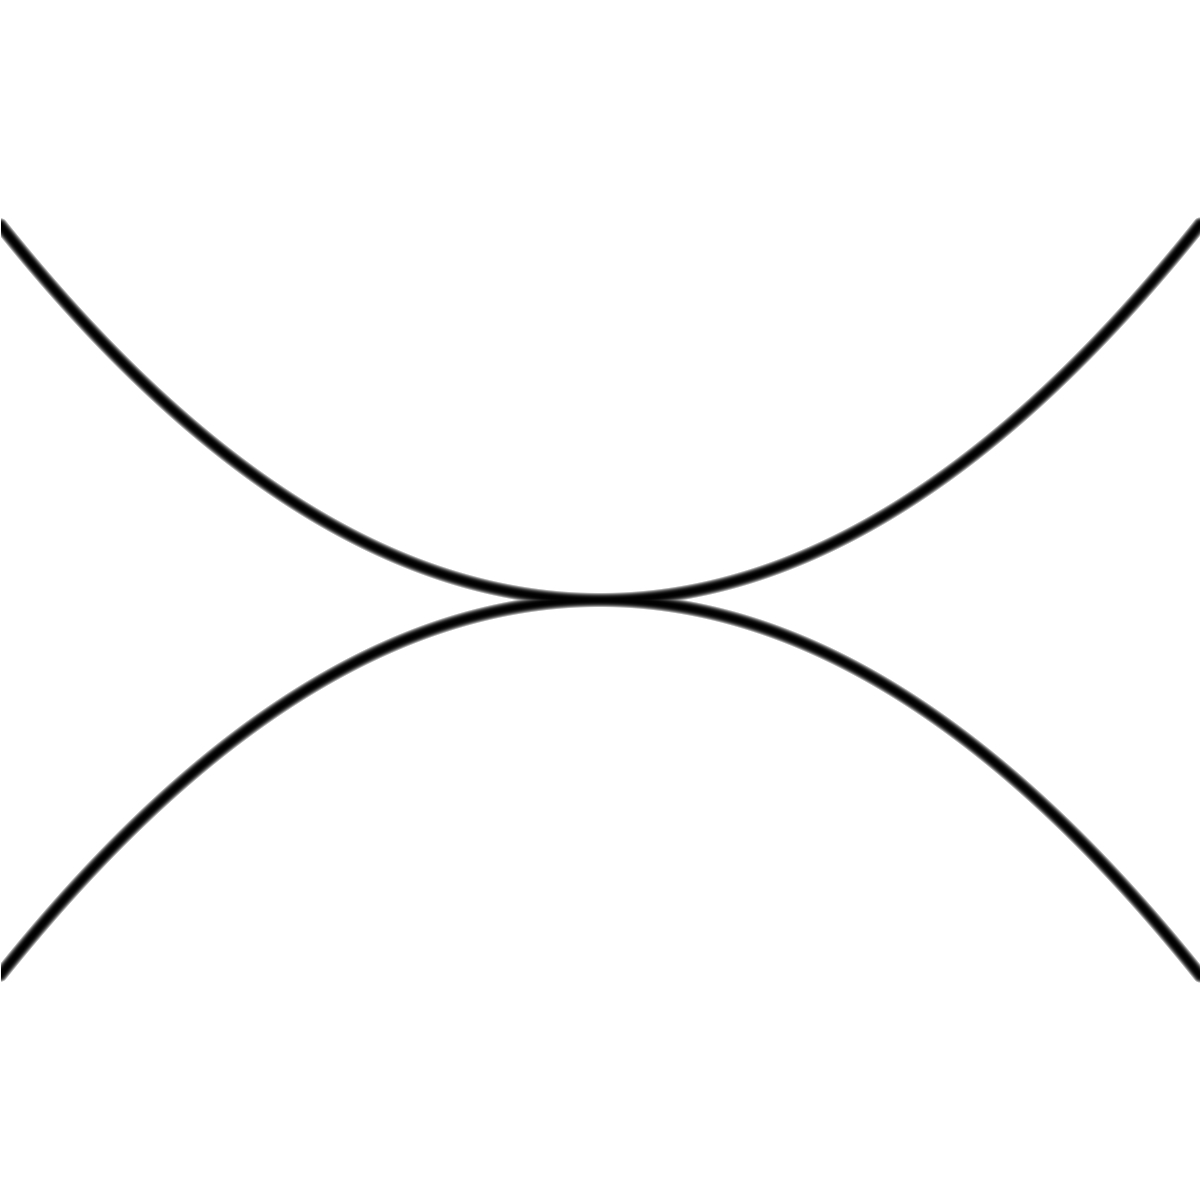
\includegraphics[width=1.4cm]{../../common/images/A3pm_cut_rot}
        \end{tabular}
        &
        \begin{tabular}{@{}c@{}}
          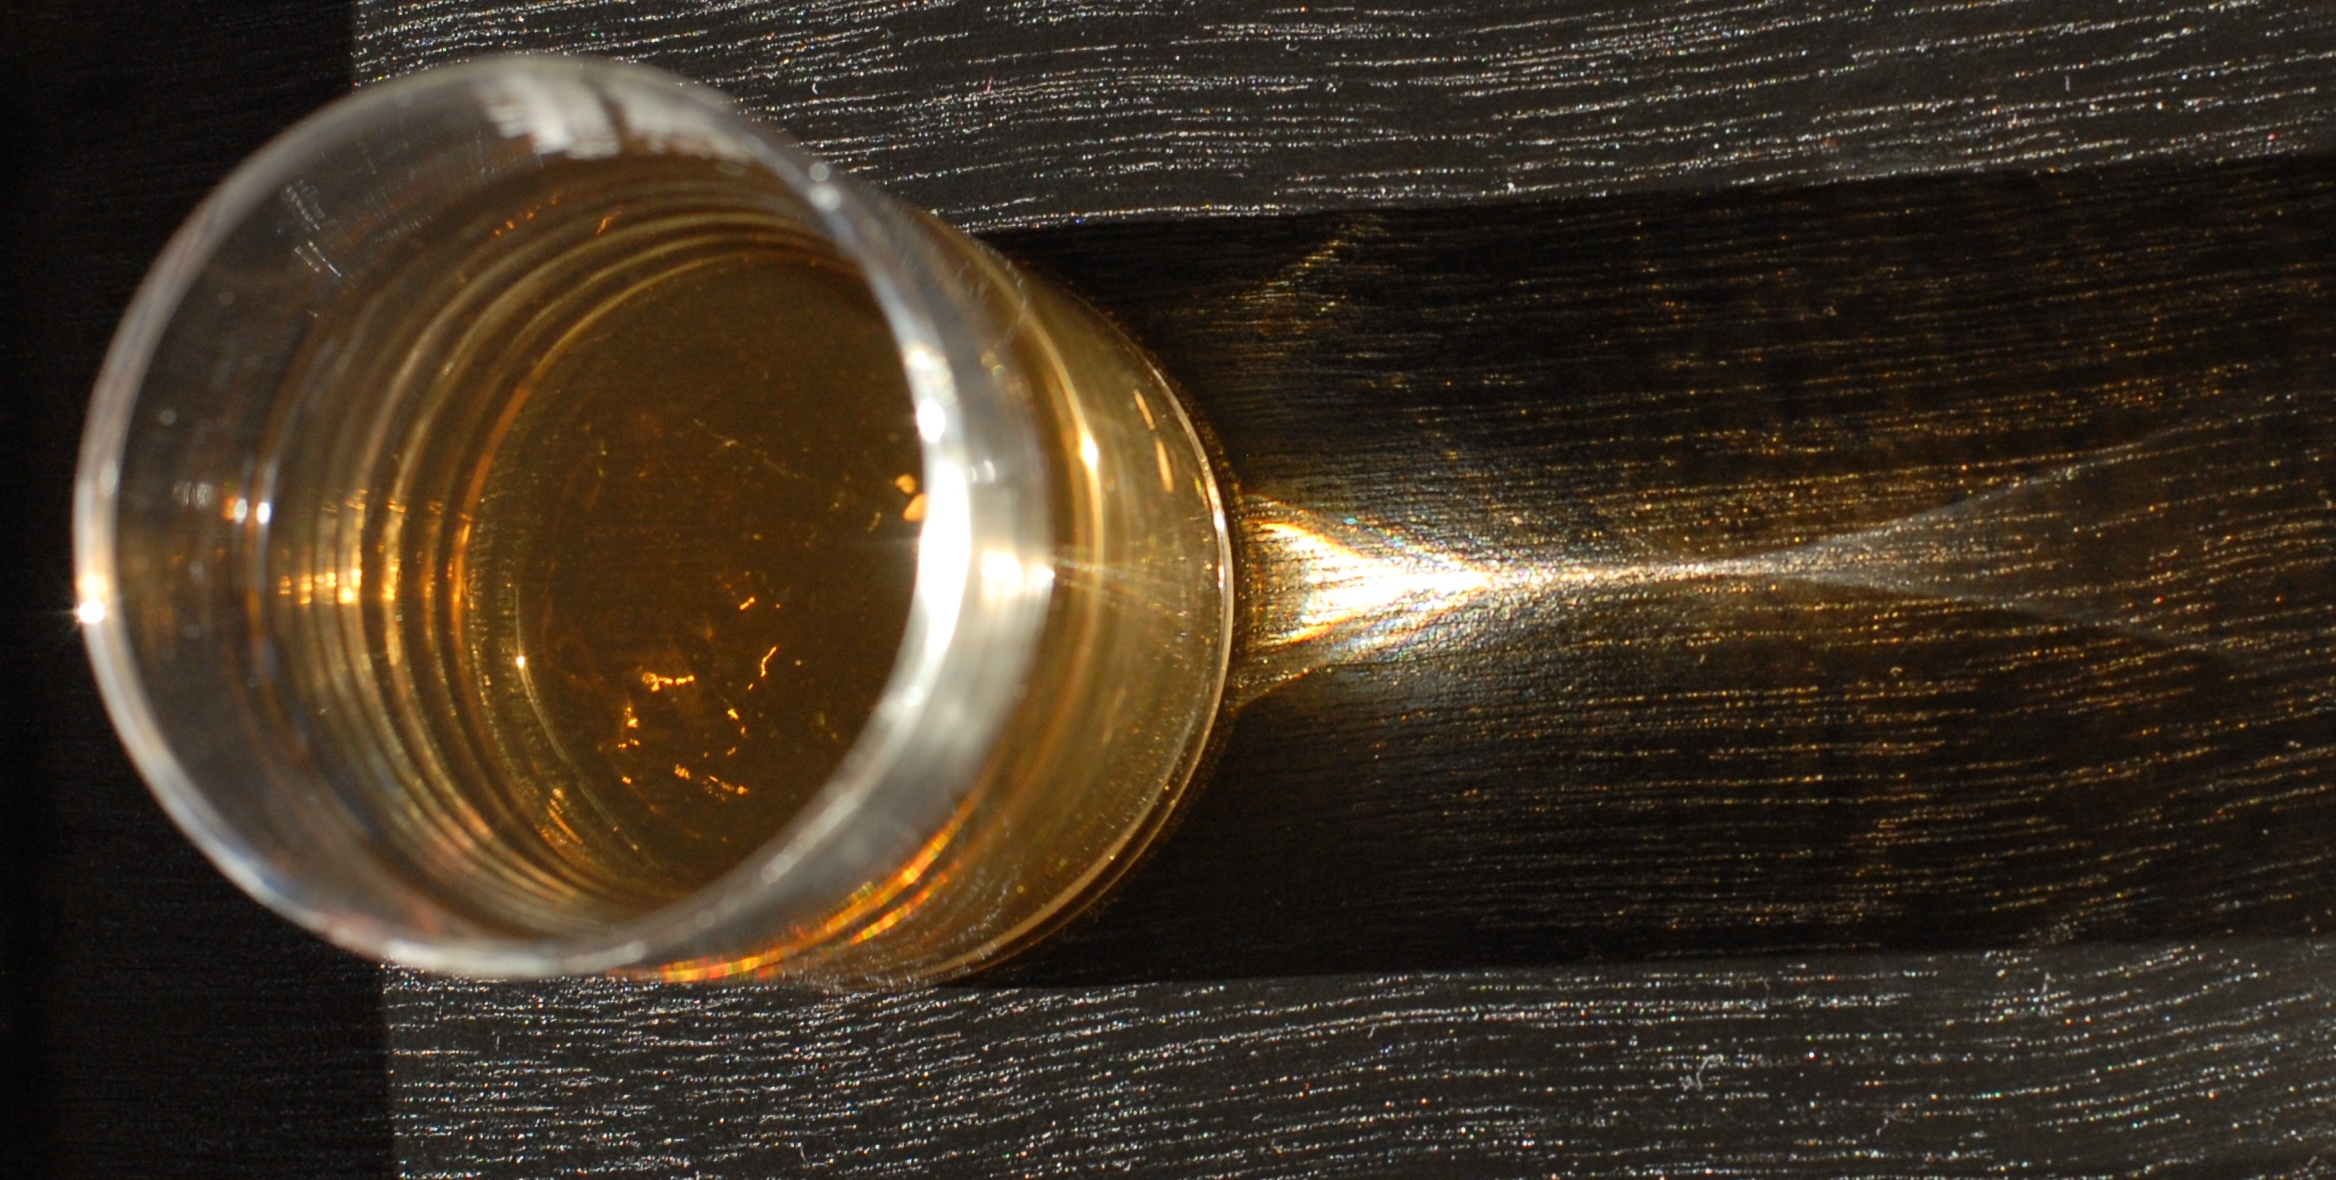
\includegraphics[height=1.4cm]{../../common/images/teeglas_detail}
        \end{tabular}
      \end{tabular}
    \end{center}
    \vspace*{-0.4em}
    Die Deformation in zwei Doppelkegel Singularitäten sieht so aus:
%    \dontshow{
    % 
    \begin{center}
      \vspace{-0.3cm}
      \begin{tabular}{@{}c@{\quad}c@{\quad}c@{}}
        \begin{tabular}{@{}c@{}}
          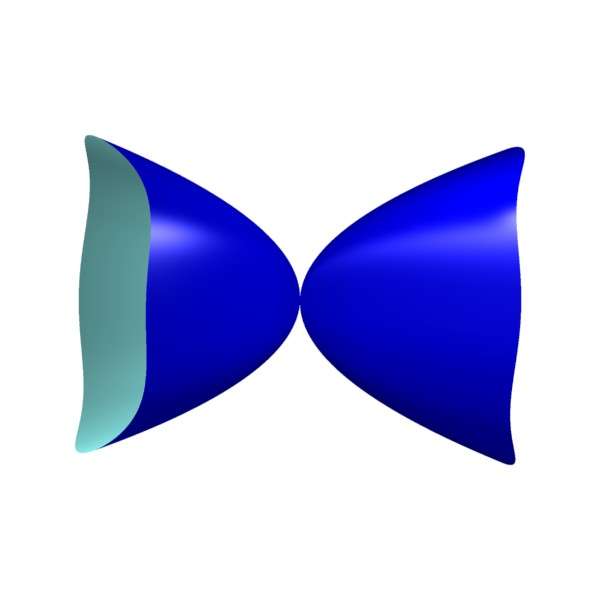
\includegraphics[width=1.2cm]{../../common/images/A3pm_0}
        \end{tabular}
        &
        \begin{tabular}{@{}c@{}}
          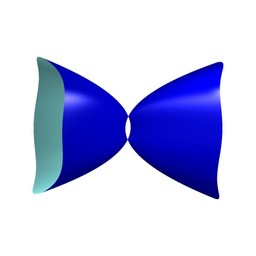
\includegraphics[width=1.2cm]{../../common/images/A3pm_1}
        \end{tabular}
        &
        \begin{tabular}{@{}c@{}}
          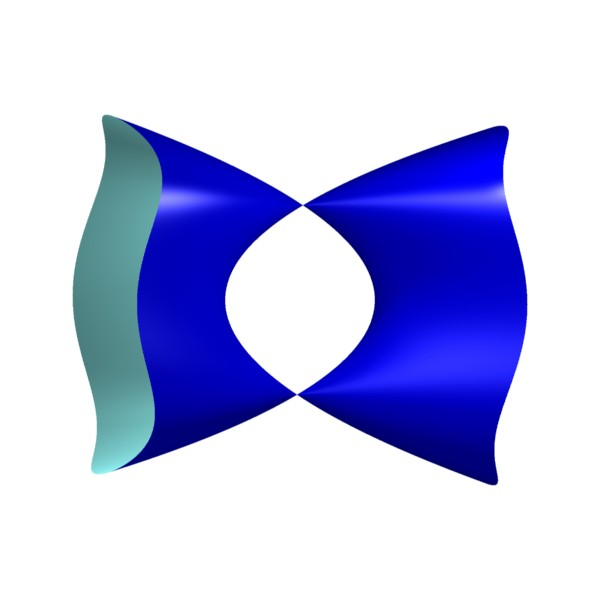
\includegraphics[width=1.2cm]{../../common/images/A3pm_2}
        \end{tabular}
      \end{tabular}
    \end{center}
%    }
 
\end{surferPage}
